\documentclass[11pt,a4paper]{article}
\usepackage[margin=25mm]{geometry}
\usepackage[T1]{fontenc}
\usepackage[utf8]{inputenc}
\usepackage{lmodern,microtype}
\usepackage{amsmath,amssymb,booktabs,array,tabularx,longtable}
\usepackage{graphicx,xcolor,caption,subcaption}
\usepackage[numbers,sort&compress]{natbib}
\usepackage{enumitem,placeins}
\usepackage{tikz}
\usetikzlibrary{arrows.meta,positioning}
\usepackage[unicode,colorlinks=true,linkcolor=black,citecolor=black,urlcolor=blue]{hyperref}
\usepackage{url}
\setlength{\emergencystretch}{2em}
\setlength{\parskip}{3pt}
\setlength{\parindent}{1.2em}
\captionsetup{font=small,labelfont=bf}
\setlist{nosep,leftmargin=*}
\newcommand{\Full}{full S4D model}
\newcommand{\cct}{\mathrm{CC}_{t}}
\newcommand{\ccs}{\mathrm{CC}_{s}}
\newcommand{\blankfield}{\mbox{}\par\vspace{5mm}}
\title{Subject-wise benchmarking of radar-to-ECG reconstruction:\\
Architectural ablations, feature-space robustness, and a reproducibility audit}
\author{}
\date{}

\begin{document}
\maketitle
\vspace{-8mm}
% Author names, affiliations, and corresponding-author details intentionally blank.

\begin{abstract}
Radar-to-electrocardiogram reconstruction is often evaluated through average waveform similarity,
although subject generalisation, beat timing and implementation details can lead to different
conclusions. We retrospectively analyse a completed benchmark of 180 training runs on the public
CR-RVS corpus: 80 convolutional baseline runs and 100 runs of a compact bidirectional diagonal
state-space model family. The processed corpus retains 134 recordings from 30 participants.
The primary resting--Valsalva--apnoea experiment uses five subject-disjoint folds and 6,278
non-overlapping test windows per model. Full-model temporal and spectral correlations are
57.46\% and 87.44\%, compared with 44.61\% and 73.70\% for our MultiResLinkNet reimplementation,
with 4.09 versus 9.22 million parameters. However, removal of feature-wise linear modulation
achieves 61.98\% temporal correlation, and the single-task variant reaches 61.74\% and exceeds
the full model in the subject-paired comparison after correction across nine tests
($p_{\mathrm{Holm}}=0.0197$). Full-model superiority to MultiResLinkNet does not survive that
correction ($p_{\mathrm{Holm}}=0.1018$). A selected-fold feature-noise stress test shows substantial
robustness, whereas held-out Tilt-up performance remains poor. A source-and-artifact audit
identifies a 125-Hz signal stream labelled as 128~Hz, limiting physiological interpretation of
the archived beat and variability metrics. These findings support further study of compact
state-space reconstruction while rejecting an additive benefit from the complete architecture.
They also show why reproducible signal processing, subject-level inference and explicit
failure analysis are necessary before waveform improvements can support clinical claims.
\end{abstract}

\noindent\textbf{Keywords:} radar-to-ECG reconstruction; diagonal state-space model;
subject-wise validation; architectural ablation; reproducibility; heart-rate variability

\section{Introduction}

Contactless cardiac sensing is attractive when long-term electrode attachment is inconvenient,
but radar and electrocardiography observe different physical quantities. Radar measures motion
and its effects on the reflected electromagnetic field, whereas the ECG records electrical
activity. Learning a transformation between the two therefore requires more than estimating
heart rate. A reconstructed trace can resemble the reference in aggregate while placing
individual beats incorrectly. The distinction matters because downstream interbeat measurements
depend on the timing of specific events, not only on the average shape of a window.

Public synchronised radar and reference datasets have made this problem experimentally
accessible. CR-RVS provides recordings under physiological interventions and postural changes
\citep{schellenberger2020}. Using this resource, Chowdhury et al. introduced MultiResLinkNet and
reported improved ECG reconstruction over convolutional alternatives \citep{chowdhury2024}.
Subsequent work has explored explicit dynamical structure, task decomposition and learnable
multiresolution representations \citep{radarode,radarodemt,lifwavnet}. These approaches motivate
the investigation of sequence models that combine local morphology with context across several
cardiac cycles. They also create a need to determine which components contribute under the same
held-out evaluation protocol.

Three distinctions govern that evaluation. First, many windows from one participant do not
provide the same evidence as observations from many participants. Subject-disjoint evaluation
addresses generalisation to new individuals, while a scenario-held-out experiment can address
condition change in people encountered during training. Second, agreement with a published
number depends on preprocessing, target scaling, model selection and aggregation; a change in
any of these can alter the comparison. Third, high spectral or temporal correlation does not
establish physiological agreement. Heart-rate variability (HRV) requires carefully defined
intervals, units and artifact handling \citep{hrvstandards,hrvoverview}.

This study examines these distinctions through a completed training campaign rather than a
newly selected collection of favourable runs. Four convolutional baseline families were trained
under a common subject-wise protocol. A second family combined an eight-channel radar
representation, learned lifting features, a bidirectional diagonal state-space bottleneck and
optional waveform, peak and interval heads. The archived implementation is S4D-based
\citep{s4d}; despite the repository name \emph{CardioMamba}, it does not implement Mamba's
input-dependent selective state-space mechanism \citep{mamba}. We use architecture-neutral
variant labels throughout the paper to make this distinction explicit.

Our contribution is an evidence-based assessment of the completed experiment. We report all
primary variants, reproduce the subject-paired tests from archived per-window results, and add
conditional bootstrap intervals for paired effect sizes. We examine scenario transfer,
feature-space perturbations and downstream peak metrics, then trace inconsistencies back to
the preprocessing and training artifacts. The resulting conclusion is narrower than a claim
of universal model superiority: compact S4D variants are promising, but the full component stack
is not the best design in this experiment, and the physiological outputs require correction
before submission as validated measurements.

\section{Related work}

\subsection{Radar-based waveform reconstruction}

MultiResLinkNet adapts an encoder--decoder architecture to reconstruct ECG from radar-derived
waveforms \citep{chowdhury2024}. Its multiresolution processing relates to MultiResUNet
\citep{multiresunet}, while U-Net, LinkNet and feature pyramid networks provide complementary
approaches to information transfer between resolutions \citep{unet,linknet,fpn}. Our baselines
are one-dimensional reimplementations of these families. The original published scores are
reference values, not results obtained with our folds. They are consequently presented
separately from within-study comparisons.

Recent radar-to-ECG methods incorporate more explicit structure. radarODE uses an
ODE-embedded reconstruction model \citep{radarode}; radarODE-MTL decomposes the task and uses
gradient alignment to address conflicts between objectives \citep{radarodemt}. LifWavNet
introduces learnable lifting and inverse-lifting operations with a multiresolution spectral
objective \citep{lifwavnet}. These methods are relevant conceptual comparators, but their
checkpoints were not rerun in the present pipeline. We make no numerical superiority claim
against them. In particular, learned lifting and multiresolution STFT losses are established
ideas, not novel primitives introduced by this study.

\subsection{State-space and multiscale representations}

Diagonal state-space layers model sequences through learned dynamical kernels with an efficient
convolutional implementation \citep{s4d}. They provide a useful alternative to attention when
the task depends on structured temporal context. The distinction from selective state spaces
is substantive: the S4D kernel used here is independent of the current input, while Mamba makes
selected dynamics input-dependent \citep{mamba}. A Transformer bottleneck \citep{attention}
serves as a within-family control, although its parameter count is not identical.

The lifting scheme separates a signal into even and odd samples followed by prediction and
update operations \citep{lifting}. Our implementation learns these operations and fuses their
features with a convolutional encoder. Efficient channel attention \citep{eca} weights the
fused representation. A separate ablation tests peak-conditioned feature-wise linear
modulation, adapted from the general FiLM formulation \citep{film}. These components offer
plausible mechanisms, but their inclusion is a hypothesis to be tested rather than evidence
that the combined network must improve.

\subsection{Physiological and statistical evaluation}

Waveform error, correlation and event detection measure different aspects of reconstruction.
Welch spectra provide a stable window-level spectral representation \citep{welch}, but
similar spectra do not guarantee correct beat placement. Likewise, an acceptable average HR
can coexist with poor successive-interval variability. Established HRV definitions
\citep{hrvstandards,hrvoverview} and agreement analysis \citep{blandaltman} therefore motivate
reporting physiology separately from waveform similarity. We use paired signed-rank tests
\citep{wilcoxon} and Holm correction \citep{holm} to avoid interpreting each ablation's
uncorrected probability as an independent discovery.

\section{Materials and methods}

\subsection{Study design and evidence freeze}

This is a retrospective analysis of a completed computational campaign. The five-stage workflow
inventoried the raw data, constructed processed recordings and folds, trained the baselines,
trained the state-space variants, and evaluated the completed runs. The final evaluation
generation, \texttt{ca226baa6c1f1ae1}, contains 80 baseline and 100 canonical experimental runs.
An additional smoke test is excluded. All 23 artifacts declared by that generation were
downloaded and checked against their recorded byte sizes and SHA-256 hashes.

For manuscript preparation, we additionally downloaded 99 pinned evidence files, including
per-window metrics for all 65 primary RVA runs, subject-level physiological summaries for
four selected models, saved waveform samples, archived modules and raw-inventory metadata. No model was retrained for
this paper. Appendix~\ref{app:provenance} identifies the exact repository revisions. This study
was not externally preregistered. The nine-comparison family was defined in the evaluation
code, while bootstrap intervals and the implementation audit were added during manuscript
preparation and are explicitly treated as retrospective analyses.

\subsection{Dataset and inclusion}

CR-RVS contains synchronised measurements acquired with a 24-GHz radar and a reference system
\citep{schellenberger2020}. The original cohort comprised 30 healthy participants: 14 male and
16 female, with a reported mean age of $30.7\pm9.9$ years. The available mirror contains 135
MATLAB recordings. Our final corpus retains 134; the only exclusion is the ECG-flatline file
\texttt{GDN0030\_4\_TiltUp.mat}. Weak radar--ECG coupling is recorded as a difficulty
indicator and is not an exclusion criterion. Table~\ref{tab:data} gives the processed counts.

\begin{table}[htbp]
\centering
\caption{Final corpus. Window counts refer to 1,024-sample windows. The physical duration of
each window is 8.192~s, as established by the sampling-rate audit.}
\label{tab:data}
\begin{tabular}{lrrr}\toprule
Scenario & Recordings & Windows, 512-sample hop & Non-overlapping windows\\\midrule
Apnoea & 24 & 1,115 & 563\\
Resting & 30 & 4,609 & 2,311\\
Tilt-down & 27 & 4,198 & 2,106\\
Tilt-up & 26 & 4,044 & 2,027\\
Valsalva & 27 & 6,791 & 3,404\\\midrule
Total & 134 & 20,757 & 10,411\\\bottomrule
\end{tabular}
\end{table}

\subsection{Signal processing and the sampling-rate discrepancy}
\label{sec:rate}

The input representation comprises raw in-phase and quadrature channels $(I,Q)$, unwrapped
phase $\phi$, displacement $d$, velocity $v$, acceleration $a$, amplitude $A$ and a
cardiac-band displacement signal $d_c$. Ellipse-based centring, rotation and axis scaling
produce corrected quadratures $(I_c,Q_c)$ for phase demodulation:
\begin{equation}
\phi[n]=\operatorname{unwrap}\!\left(\operatorname{atan2}(Q_c[n],I_c[n])\right),
\qquad d[n]=\frac{\lambda}{4\pi}\phi[n].
\end{equation}
Here $\lambda=12.49135$~mm. Velocity and acceleration use Savitzky--Golay derivatives with
a nine-sample window and polynomial order three at the source sampling rate. The amplitude
channel is $\sqrt{(I-\bar I)^2+(Q-\bar Q)^2}$; $d_c$ is a zero-phase fourth-order
Butterworth-filtered displacement in the 0.8--20-Hz band. The ECG lead-I target is processed
with a 50-Hz notch and a 0.5--40-Hz bandpass. No additional ECG-guided temporal shift is
applied in the model-input path. These are the implemented operations; an earlier planning
document's polynomial-detrending description is not treated as evidence of execution.

The intended output rate was 128~Hz. However, the processing function selects an integer
decimation factor $q=\operatorname{round}(f_{\mathrm{source}}/128)$. Every inventoried source
recording has $f_{\mathrm{source}}=2{,}000$~Hz, giving $q=16$ and an actual rate of
125~Hz. The metadata nevertheless stores 128~Hz. For all 134 retained recordings, the saved
length is exactly $\lceil N_{\mathrm{source}}/16\rceil$, independently confirming the
discrepancy. Thus a 1,024-sample window spans 8.192~s rather than 8~s.

We preserve archived results instead of relabelling them as corrected experiments. Temporal
correlation and sample-wise errors depend on sample values, not the assigned time axis.
The reported spectral correlation compares the same Welch-bin arrays for both signals and
is also invariant to a shared rate-label change in this implementation. In contrast, peak
filtering, refractory intervals, interval thresholds, frequency labels and HR/HRV conversion
use the nominal rate. Physiological metrics are therefore labelled \emph{nominal} and are
not validated physical measurements. Appendix~\ref{app:timing} derives the purely algebraic
unit correction and explains why it does not replace rerunning the detector.

\subsection{Targets, normalisation and windows}

The ECG is normalised separately within each complete recording: it is centred and scaled,
clipped at its 0.5th and 99.5th percentiles, and linearly mapped to $[-1,1]$. This defines a
shape-reconstruction target, not ECG voltage calibration. Because target normalisation uses
the complete reference recording, the benchmark does not establish recovery of its absolute
amplitude in a deployment without reference electrodes.

The auxiliary peak target is a Gaussian heatmap with standard deviation three samples around
detected events. The RR target interpolates intervals between successive detected events,
retaining nominal intervals between 300 and 2,000~ms and expressing the target in seconds.
Input-channel means and standard deviations are estimated from at most 4,000 sampled training
windows per split. Normalised inputs are clipped to $[-8,8]$. Training augmentation adds
Gaussian noise of standard deviation 0.01 with probability 0.5 and multiplies the inputs by
a gain drawn from $\mathcal N(1,0.1^2)$ with probability 0.3.

Windows have length 1,024 samples. Training uses a hop of 512 samples; validation and test
use only starts divisible by 1,024. These restrictions prevent overlap between evaluated
windows, while subject partitioning prevents a participant's training windows from appearing
in the primary test split.

\subsection{Partitions and experiment matrix}

Subjects are sorted by the number of available scenarios and then recording duration, both
descending, and assigned round-robin to five groups. For fold $f$, group $f$ is held out,
group $(f+1)\bmod5$ is used for validation, and the remaining three groups train the model.
The RVA task combines resting, Valsalva and apnoea and contains 6,278 non-overlapping windows
across its held-out folds for each model. All primary models use the same partitions.

The 80 baseline runs comprise four models, four tasks (the three individual scenarios plus
RVA), and five folds. The 100 experimental runs comprise nine RVA variants across five folds
(45), the full model on three individual scenarios across five folds (15), the full model on
all five scenarios across five folds (5), 30 leave-one-subject-out (LOSO) runs, and five
held-out-scenario runs. LOSO holds one subject out for testing, reserves the next indexed
subject for validation, and trains on the other 28.

In held-out-scenario evaluation, one scenario is the test condition, the next in a fixed
cyclic order is validation, and the other three train the model. Participants can appear
across these condition partitions. This experiment tests transfer to an unseen condition
within the available participant pool; it does not test simultaneous transfer to a new
condition and new subjects.

\subsection{Model architecture}

Figure~\ref{fig:architecture} summarises the implemented network. A pointwise convolution mixes
the eight radar channels into 32 features, followed by a convolutional stem. Four MultiRes
encoder stages use nominal widths 32, 64, 128 and 256. The resulting channel counts are
51, 105, 212 and 426, at sequence lengths 1,024, 512, 256 and 128 before pooling.
Residual paths carry features to an additive decoder with four upsampling stages.

\begin{figure}[htbp]
\centering
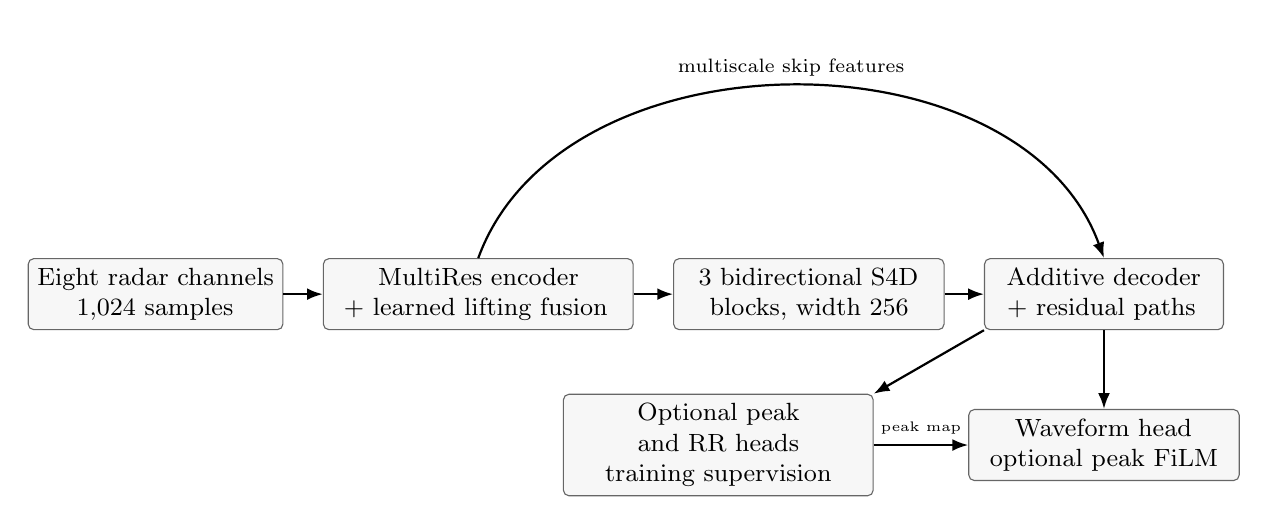
\begin{tikzpicture}[node distance=5mm,box/.style={draw=black!60,rounded corners=2pt,
fill=black!3,align=center,font=\small,minimum height=9mm},arr/.style={-{Latex[length=2mm]},thick}]
\node[box,text width=30mm] (input) {Eight radar channels\\1,024 samples};
\node[box,text width=37mm,right=of input] (enc) {MultiRes encoder\\+ learned lifting fusion};
\node[box,text width=32mm,right=of enc] (ssm) {3 bidirectional S4D\\blocks, width 256};
\node[box,text width=28mm,right=of ssm] (dec) {Additive decoder\\+ residual paths};
\node[box,text width=32mm,below=10mm of dec] (wave) {Waveform head\\optional peak FiLM};
\node[box,text width=37mm,left=12mm of wave] (aux) {Optional peak and RR heads\\training supervision};
\draw[arr] (input)--(enc);\draw[arr] (enc)--(ssm);\draw[arr] (ssm)--(dec);
\draw[arr] (dec)--(wave);\draw[arr] (dec.south west)--(aux.north east);
\draw[arr] (aux)--node[above,font=\tiny]{peak map}(wave);
\draw[arr] (enc.north) to[out=70,in=110] node[above,font=\scriptsize]{multiscale skip features} (dec.north);
\end{tikzpicture}
\caption{Implemented reconstruction family. The single-task variant removes both auxiliary
heads and FiLM; the no-FiLM variant retains the heads. The temporal bottleneck uses S4D,
not an input-dependent selective Mamba layer.}
\label{fig:architecture}
\end{figure}

The lifting branch starts with a projection at the input resolution, followed by three
learned lifting units. Each splits its input into even and odd samples and computes
\begin{equation}
d_i=x_{o,i}-P_i(x_{e,i}),\qquad c_i=x_{e,i}+U_i(d_i),
\end{equation}
where $P_i$ and $U_i$ are small convolutional networks. Projected concatenations of
$(c_i,d_i)$ are fused with matching-resolution convolutional features using a pointwise
convolution and channel attention. These learned features are not assumed to be orthogonal
wavelets, and the decoder does not perform an inverse lifting transform.

After the final pooling operation, features have length 64 and are projected to width 256.
Three bidirectional S4D blocks process this sequence. For feature $h$ and complex state $j$,
the diagonal dynamics are parameterised as
\begin{equation}
A_{hj}=-\exp(a_{hj})+\mathrm{i}\omega_{hj},\qquad
\Delta_h=\exp(\delta_h),
\end{equation}
with 32 complex states representing the configured state dimension of 64. The convolution
kernel is
\begin{equation}
K_h[\ell]=2\operatorname{Re}\sum_j C_{hj}
\frac{\exp(\Delta_h A_{hj})-1}{A_{hj}}
\exp(\ell\Delta_h A_{hj}).
\label{eq:s4d}
\end{equation}
Each direction convolves this kernel with the normalised features and adds a learned direct
term. Forward and reversed-sequence outputs are concatenated and projected; residual
connections and a twofold-expanded GELU feed-forward block complete the layer. The code uses
FFT convolution with sequence-dependent $O(L\log L)$ convolution cost, plus kernel formation,
and does not establish a linear-time streaming implementation. Bidirectional processing and
zero-phase preprocessing also make the evaluated pipeline noncausal.

The waveform head uses a hyperbolic tangent. Optional heads produce a peak logit and a
positive RR estimate. In the full variant, the predicted peak probability conditions waveform
features through
\begin{equation}
\widetilde F=(1+\tanh\gamma(p))\odot F+\beta(p),
\end{equation}
with gradients flowing through the conditioning pathway. The Transformer control uses three
encoder layers, width 256, eight heads, a twofold-expanded feed-forward sublayer and learned
positional embeddings.

\subsection{Objectives and training}

The composite objective combines Huber error \citep{huber}, multiresolution STFT discrepancy
in the spirit of waveform-generation losses \citep{wavegan}, waveform correlation,
peak-weighted absolute error, focal peak loss \citep{focal}, and RR absolute error:
\begin{align}
\mathcal L={}&\mathcal L_H+0.5\mathcal L_{\mathrm{STFT}}+
0.3(1-r(y,\hat y))+0.5\mathcal L_{\mathrm{pw}}\nonumber\\
&+0.3\mathcal L_{\mathrm{peak}}+0.1\mathcal L_{\mathrm{RR}}.
\label{eq:loss}
\end{align}
The Huber threshold is 0.1. STFT resolutions are 64, 128 and 256 samples, with Hann windows
and quarter-window hops; each resolution combines relative spectral convergence and
log-magnitude error. Peak-weighted error uses weights $1+4p_{\mathrm{target}}$.
The focal parameters are $\alpha=0.75$ and $\gamma=2$. Terms for absent auxiliary heads are
omitted. Single-task training therefore retains peak-weighted waveform supervision; it is
single-output training, not training without peak-derived labels. MultiResLinkNet-based
variants additionally use the implemented auxiliary deep-supervision outputs with weight 0.2.

Baselines use displacement only, MSE, targets in $[0,1]$, a maximum of 120 epochs, batch size
64, initial learning rate $5\times10^{-4}$ and early-stopping patience 20 on validation loss.
The experimental variants use targets in $[-1,1]$, at most 150 epochs, batch size 48,
learning rate $8\times10^{-4}$ and patience 25 on validation temporal correlation, with a
minimum of 40 epochs. Both use AdamW \citep{adamw}, weight decay $10^{-4}$, gradient clipping
at norm 1 and cosine learning-rate decay to $10^{-6}$. Seeds are $1337+f$ for fold $f$.
The hardware is Kaggle dual Tesla T4; saved environments record PyTorch 2.10.0 with CUDA 12.8.

These training differences matter. The baseline-to-L2 comparison changes more than the loss:
target convention, training budget and checkpoint selection also change. It is consequently
a protocol comparison, not an isolated causal estimate of the composite objective. L5--L10
provide more closely matched architectural comparisons within the experimental protocol.

Training runs in isolated process chunks to release memory. Checkpoints preserve model,
optimiser, scheduler, random-state and batch-cursor information. Numerical recovery restores
a finite checkpoint and reduces the learning rate by a factor of 0.25; automatic mixed
precision is disabled after the second recovery. The configured maximum is three recoveries.
The campaign contains more than one engine revision, so the archived per-run configurations
and recovery records, rather than a single current engine file, define execution provenance.

\subsection{Metrics and statistical analysis}

For each window, temporal and spectral correlations are
\begin{equation}
\cct=100\,r(y,\hat y),\qquad
\ccs=100\,r(\operatorname{Welch}(y),\operatorname{Welch}(\hat y)),
\end{equation}
using Welch segments of up to 256 samples. Constant signals receive zero correlation.
MAE and MSE are compared on the $[0,1]$ scale; experimental-model errors originally measured
on $[-1,1]$ are divided by two and four, respectively. Temporal relative RMSE is omitted
from direct comparisons because an additive target offset changes its denominator and the
stored scalar cannot be converted exactly without the underlying target.

Headline values are arithmetic means of five fold-level window means. Their reported
standard deviations describe fold variability, not confidence intervals from independent
training repetitions. For paired tests, windows are first averaged within participant and
model, yielding 30 paired participant means. We reproduce the two-sided Wilcoxon tests
for full L9 against nine specified comparators and apply Holm correction at 0.05.
FPN, U-Net and LinkNet are reported descriptively and were not in that nine-test family.

To characterise effect size, we resample the 30 paired participant differences 20,000 times
and report percentile intervals for their mean (seed 20260907). These added intervals are
unadjusted, retrospective and conditional on the existing fitted models and folds. They
do not capture training-seed uncertainty, and shared training sets induce dependence not
represented by simple participant resampling. Their exclusion of zero therefore does not
override a nonsignificant multiplicity-adjusted signed-rank test.

Peak and interval analyses concatenate consecutive non-overlapping predictions within each
recording, never across recordings. The detector bandpasses the trace at nominal 5--25~Hz,
squares its first difference, smooths over approximately 100 nominal milliseconds and
finds peaks above 0.35 times the 98th percentile of that energy, with a 250-ms nominal
refractory period. A greedy one-to-one nearest-event match uses a 100-ms nominal tolerance.
This is an energy-event detector, not independently annotated ECG R-peak truth. Precision,
recall and F1 quantify agreement between detections on the predicted and reference traces.

RR intervals outside nominal 300--2,000~ms are removed. Mean HR is the average of
$60{,}000/RR_k$, and RMSSD is the root mean square of successive retained RR differences.
Records with insufficient events return missing interval metrics. Within-participant means
across recordings are used for the main physiological table and descriptive Bland--Altman
plots \citep{blandaltman}. They are not interchangeable with a mean of absolute
recording-level errors, which is also stored in the run summaries.

\subsection{Feature-space robustness and computational budget}

The archived stress test evaluates the first sorted primary checkpoint (fold 0) on the first
800 test windows in dataset order. The same window order is used for the two models, but
random perturbation seeds differ by model. Gaussian noise is added after input
normalisation and clipping, with variance determined from the mean input power across
channels and time. Additional cases add a shared sinusoid at nominal 0.30~Hz or zero one
normalised channel. These tests stress the model's feature representation: independent
noise on derived phase, displacement and derivatives is not equivalent to perturbing raw
I/Q and recomputing physically consistent channels. No corruption-specific retraining is
performed.

Parameter counts include all trainable tensors. The archived operation estimates use
PyTorch's operation counter on a single-window forward pass. Because operator coverage
for complex arithmetic, kernel generation and FFTs is not established, these values are
reported as \emph{counted operations}, not audited total algorithmic FLOPs. Single-call
latencies include substantial warmup outliers and are not used to claim a validated speedup.

\section{Results}

\subsection{Primary reconstruction performance}

Table~\ref{tab:primary} reports every primary model. The \Full{} achieves temporal
correlation of $57.46\pm9.89\%$ and spectral correlation of $87.44\pm2.45\%$. The corresponding
MultiResLinkNet rerun scores are $44.61\pm21.39\%$ and $73.70\pm20.79\%$. The differences in
mean temporal and spectral correlation are 12.85 and 13.74 percentage points. MAE and MSE
decrease only slightly, from 0.1657 to 0.1649 and from 0.0427 to 0.0424, respectively.
Thus the gain in correlation does not imply an equally large gain in sample-wise error.

\begin{table}[htbp]
\centering\small
\caption{Primary RVA results. Correlations are percentages, reported as mean $\pm$ sample
SD of five fold means. All models evaluate the same 6,278 windows from 30 participants.
MAE/MSE use the common $[0,1]$ comparison scale. M denotes millions of parameters.}
\label{tab:primary}
\setlength{\tabcolsep}{4pt}
\begin{tabular}{lrrrrr}\toprule
Model & MAE & MSE & $\cct$ & $\ccs$ & Params (M)\\\midrule
FPN & 0.1575 & 0.0404 & 53.27 $\pm$ 14.43 & 82.65 $\pm$ 5.67 & 2.237 \\
U-Net & 0.1660 & 0.0433 & 28.71 $\pm$ 26.11 & 47.06 $\pm$ 46.31 & 12.211 \\
LinkNet & 0.1559 & 0.0395 & 48.55 $\pm$ 10.18 & 79.33 $\pm$ 6.17 & 2.775 \\
MultiResLinkNet & 0.1657 & 0.0427 & 44.61 $\pm$ 21.39 & 73.70 $\pm$ 20.79 & 9.219 \\
L2: composite loss & 0.1565 & 0.0379 & 52.82 $\pm$ 8.13 & 87.84 $\pm$ 2.53 & 9.219 \\
L3: eight inputs & 0.1625 & 0.0405 & 59.62 $\pm$ 8.98 & 87.55 $\pm$ 3.37 & 9.222 \\
L4: inputs + loss & 0.1542 & 0.0377 & 56.44 $\pm$ 12.69 & 87.71 $\pm$ 3.36 & 9.222 \\
L5: no lifting & 0.1620 & 0.0398 & 56.91 $\pm$ 7.06 & 89.10 $\pm$ 2.02 & 3.522 \\
L6: no SSM & 0.1622 & 0.0416 & 51.52 $\pm$ 10.13 & 87.21 $\pm$ 4.92 & 3.099 \\
L7: single-task & 0.1628 & 0.0412 & 61.74 $\pm$ 7.11 & 88.81 $\pm$ 2.51 & 4.081 \\
L8: no FiLM & 0.1715 & 0.0440 & 61.98 $\pm$ 7.41 & 89.16 $\pm$ 2.89 & 4.088 \\
L9: full S4D model & 0.1649 & 0.0424 & 57.46 $\pm$ 9.89 & 87.44 $\pm$ 2.45 & 4.091 \\
L10: Transformer & 0.1701 & 0.0441 & 50.89 $\pm$ 7.72 & 87.59 $\pm$ 2.50 & 4.549 \\
\bottomrule\end{tabular}

\end{table}

The largest temporal and spectral correlations are obtained by L8 without FiLM, at 61.98\%
and 89.16\%, followed by the L7 single-task model at 61.74\% and 88.81\%. Their waveform
errors tell a different story: no-FiLM has the highest MAE among the primary variants,
while L4, which combines eight inputs and the composite objective on the MultiResLinkNet
backbone, achieves the lowest MAE and MSE. Model selection would therefore change if absolute
waveform error replaced correlation as the primary objective.

Among the strict convolutional reruns, FPN has the highest temporal correlation, 53.27\%,
and uses only 2.24 million parameters. The full S4D model exceeds that correlation by
4.19 points but is larger. Its parameter advantage applies specifically to MultiResLinkNet
and U-Net, not to all convolutional alternatives. Figure~\ref{fig:folds} shows the broad
fold variability that accompanies these mean comparisons. Appendix~\ref{app:qualitative}
shows matched waveform examples selected by a fixed within-fold quantile rule.

\begin{figure}[htbp]\centering
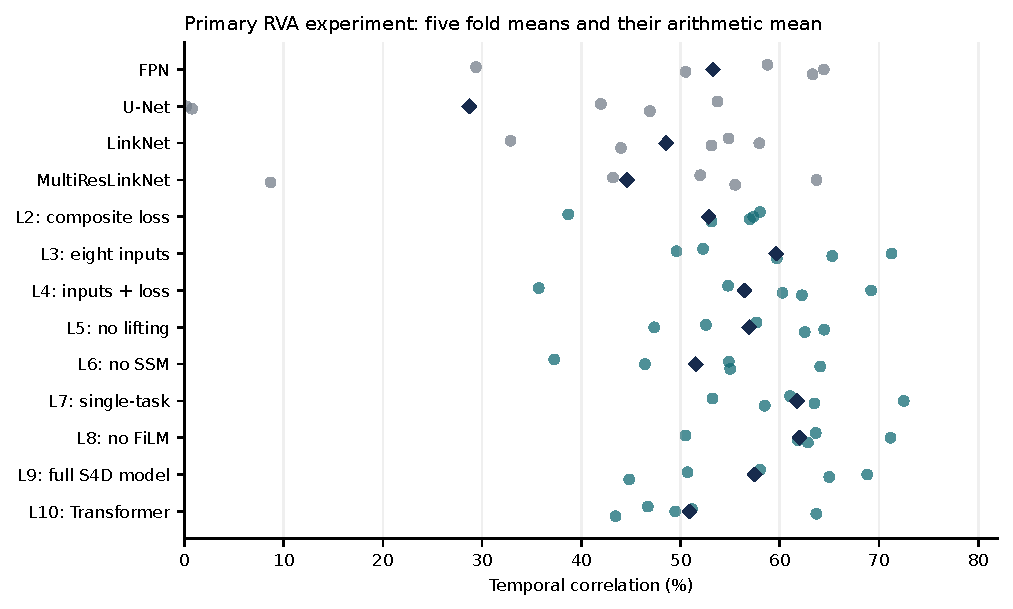
\includegraphics[width=.94\linewidth]{figures/fold_performance.pdf}
\caption{Temporal correlation for all primary variants. Circles show the five fold means;
diamonds show their arithmetic mean. Folds share training participants and are not independent
seed repetitions. The weak MultiResLinkNet fold contributes strongly to its overall deficit.}
\label{fig:folds}
\end{figure}

The published combined-scenario MultiResLinkNet values are 61.86\% temporal and 79.96\%
spectral correlation \citep{chowdhury2024}. Our reproduction gate fails because the rerun's
temporal correlation is 17.25 points below the published value and the baseline ranking
differs. This discrepancy does not identify its cause. Our partitions, preprocessing,
implementation and training settings differ from the published experiment. In particular,
the result cannot establish that the original evaluation suffered from leakage. Full L9
also remains below the published temporal value, while no-FiLM is numerically close to it;
neither constitutes a controlled comparison against the published trained model.

\subsection{Participant-level effects and ablations}

Table~\ref{tab:stats} reproduces the nine participant-paired tests. Full L9 is better than
MultiResLinkNet on 20 of 30 participant means. Its median difference is 3.21 points,
considerably smaller than the mean difference of 12.63 points. This asymmetry is consistent
with large gains concentrated in a subset of poorly reconstructed baseline subjects.
The raw signed-rank probability is 0.0145, but the Holm-adjusted value is 0.1018.

\begin{table}[htbp]\centering\small
\caption{Paired temporal-correlation differences, full L9 minus comparator, across 30
participants. Positive values favour L9. Bootstrap intervals are retrospective, unadjusted
95\% percentile intervals for the mean difference conditional on the fitted models.
The signed-rank tests form one family of nine comparisons.}
\label{tab:stats}
\setlength{\tabcolsep}{4pt}
\begin{tabular}{lrrrr}\toprule
Comparator & Median $\Delta$ & Mean $\Delta$ [95\% interval] & $p$ & $p_{\mathrm{Holm}}$\\\midrule
L7: single-task & -2.26 & -4.88 [-8.59, -1.86] & 0.0022 & 0.0197 \\
L10: Transformer & +5.01 & +5.95 [1.36, 10.44] & 0.0120 & 0.0964 \\
MultiResLinkNet & +3.21 & +12.63 [3.69, 22.27] & 0.0145 & 0.1018 \\
L8: no FiLM & -3.62 & -4.87 [-8.95, -1.35] & 0.0221 & 0.1326 \\
L6: no SSM & +5.34 & +6.06 [0.54, 11.61] & 0.0549 & 0.2746 \\
L2: composite loss & +3.84 & +4.61 [-0.89, 9.62] & 0.0606 & 0.2746 \\
L3: eight inputs & +0.31 & -2.32 [-6.51, 1.25] & 0.6120 & 1.0000 \\
L4: inputs + loss & +1.27 & +1.52 [-4.09, 7.19] & 0.6263 & 1.0000 \\
L5: no lifting & -0.52 & +0.37 [-5.32, 5.90] & 0.7766 & 1.0000 \\
\bottomrule\end{tabular}

\end{table}

The only comparison below 0.05 after correction favours the single-task model over L9.
The full-minus-single-task median difference is $-2.26$ points, with a mean of $-4.88$
and a conditional bootstrap interval of $[-8.59,-1.86]$. Full L9 is better on only six
participant means. Removing FiLM also improves the overall correlation, but the corresponding
adjusted probability is 0.1326. Figure~\ref{fig:pairs} illustrates the direction and
heterogeneity of the paired results.

\begin{figure}[htbp]\centering
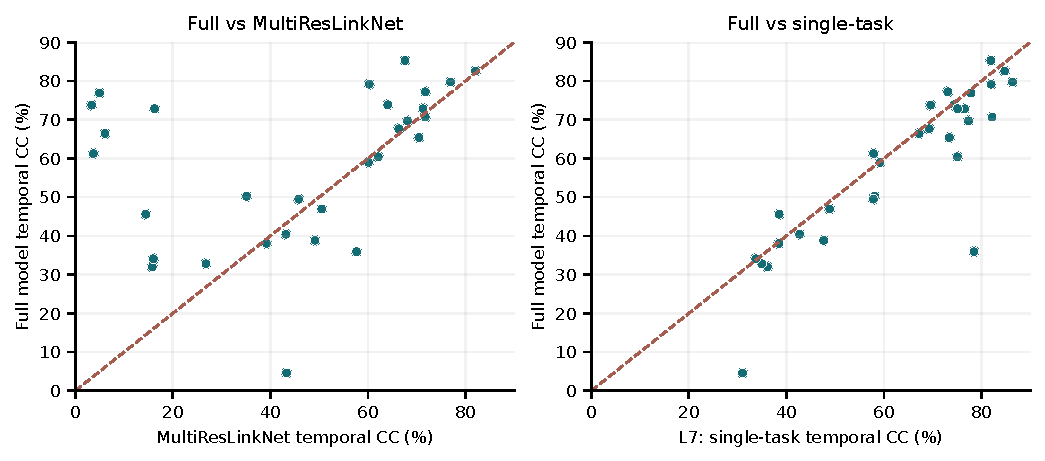
\includegraphics[width=\linewidth]{figures/subject_pairs.pdf}
\caption{One point per participant, using the mean of their held-out window correlations.
Points above the diagonal favour full L9. Large improvements over some weak MultiResLinkNet
subjects contrast with the more consistent single-task advantage.}
\label{fig:pairs}
\end{figure}

Replacing the S4D bottleneck with convolutions reduces mean temporal correlation to 51.52\%;
the Transformer control reaches 50.89\%. Both contrasts favour full L9 on average, but
neither survives Holm correction. Removing lifting changes the mean by only $-0.56$ points,
with no evidence of a consistent paired advantage. These findings support investigation of
the S4D bottleneck but do not establish that the lifting branch is necessary. Because L2--L4
also differ from the strict baseline in optimisation and target convention, their gains
cannot be assigned exclusively to input features or the objective.

\subsection{Scenario and participant generalisation}

The full model's separate-scenario temporal/spectral correlations are 56.66/87.52\% for
resting, 51.47/86.69\% for Valsalva and 45.07/82.56\% for apnoea. Its temporal correlation
improves on the MultiResLinkNet rerun by 6.73 points in resting and 3.32 points in apnoea,
while Valsalva is effectively unchanged ($-0.014$ points). MAE is worse than MultiResLinkNet
in resting and apnoea despite their improved correlations. Full-model gains therefore depend
on both condition and metric.

\begin{table}[htbp]\centering\small
\caption{Full-model generalisation results. Five-fold and LOSO rows are subject-disjoint.
Scenario-held-out rows permit participant overlap between training and testing; each is one
fitted model and tests condition transfer only.}
\label{tab:generalisation}
\begin{tabular}{llrrr}\toprule
Protocol & Test domain & Fits & $\cct$ (\%) & $\ccs$ (\%)\\\midrule
Five-fold & All five scenarios & 5 & 56.02 & 86.71\\
LOSO & All five scenarios & 30 & 54.94 & 86.90\\\midrule
Scenario-held-out & Apnoea & 1 & 67.99 & 91.07\\
Scenario-held-out & Resting & 1 & 75.19 & 94.06\\
Scenario-held-out & Tilt-down & 1 & 73.35 & 93.10\\
Scenario-held-out & Tilt-up & 1 & 28.70 & 81.69\\
Scenario-held-out & Valsalva & 1 & 77.58 & 94.59\\\bottomrule
\end{tabular}
\end{table}

The five-scenario and LOSO results are similar in spectral correlation and somewhat below
RVA in temporal correlation (Table~\ref{tab:generalisation}). Held-out Tilt-up is a distinct
failure, with 28.70\% temporal correlation despite 81.69\% spectral correlation. Stronger
scores on the other held-out scenarios should not be interpreted as evidence that condition
transfer is easier than unseen-subject reconstruction: the training populations and
validation conditions differ across protocols.

\subsection{Peak detection and nominal physiological measurements}

Table~\ref{tab:clinical} uses equal participant weighting after averaging recordings within
each participant. Full L9 improves event F1 from 0.627 to 0.813 relative to MultiResLinkNet.
Precision increases from 0.783 to 0.894, and recall from 0.555 to 0.764. The single-task and
no-FiLM models reach higher F1 values of 0.848 and 0.850. These are agreement measures
between algorithmically detected events; the permissive nominal matching tolerance and
absence of adjudicated event labels limit a claim of precise R-peak recovery.

\begin{table}[htbp]\centering\small
\caption{Participant-level event and nominal physiological results on RVA. Event metrics
are averaged within participant and then across participants. HR and RMSSD errors use the
archived 128-Hz interpretation and are not physically validated values; see
Section~\ref{sec:rate}. These aggregation weights differ from the per-fold recording-MAE
summaries used in the original ablation table.}
\label{tab:clinical}
\begin{tabular}{lrrrrr}\toprule
Model & F1 & Precision & Recall & HR MAE & RMSSD MAE \\ & & & & (nominal bpm) & (nominal ms)\\\midrule
MultiResLinkNet & 0.627 & 0.783 & 0.555 & 13.61 & 271.28 \\
L9: full S4D model & 0.813 & 0.894 & 0.764 & 3.20 & 201.42 \\
L7: single-task & 0.848 & 0.892 & 0.823 & 2.98 & 179.24 \\
L8: no FiLM & 0.850 & 0.902 & 0.819 & 2.79 & 169.01 \\
\bottomrule\end{tabular}

\end{table}

The archived full-model HR error is 3.20 nominal bpm compared with 13.61 for MultiResLinkNet.
RMSSD error remains 201.42 nominal ms, despite decreasing from 271.28. The full-model
agreement plots show substantially narrower HR differences but large residual RMSSD
disagreement (Fig.~\ref{fig:agreement}). Because these plots use participant means rather
than individual beat intervals, they describe agreement of aggregated summaries and do not
establish per-beat accuracy.

\begin{figure}[htbp]\centering
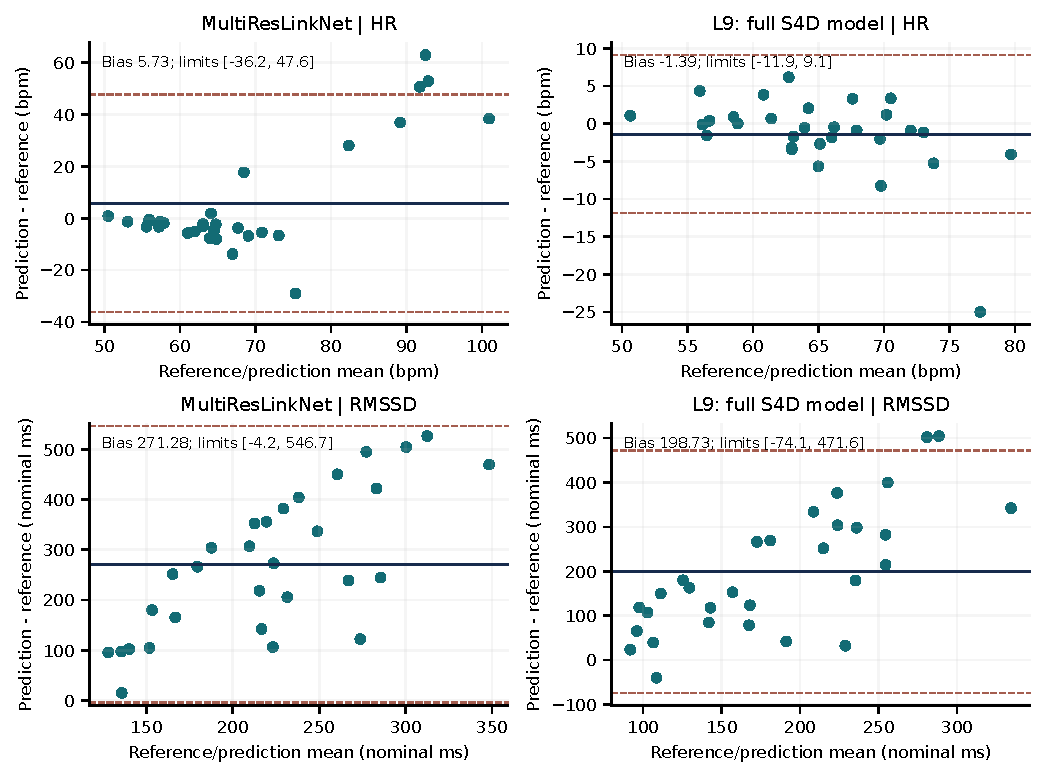
\includegraphics[width=.96\linewidth]{figures/agreement.pdf}
\caption{Descriptive Bland--Altman plots for participant-averaged physiological summaries,
$n=30$ per panel. Solid lines show bias and dashed lines show bias $\pm1.96$ population-SD
of the observed differences. All axes use archived nominal timing. No acceptance threshold
or clinical equivalence test is implied.}
\label{fig:agreement}
\end{figure}

\subsection{Feature-space perturbations}

On the selected 800-window fold subset, clean temporal correlations are 63.01\% for full
L9 and 57.49\% for MultiResLinkNet. At 12-dB feature noise they become 60.51\% and 8.92\%,
corresponding to 96.04\% and 15.52\% retention of the clean correlation. At 0~dB they are
40.83\% and 1.55\%, respectively (Fig.~\ref{fig:robustness}). A shared sinusoidal drift of
amplitude 0.5 produces 59.02\% and 47.55\% temporal correlation.

\begin{figure}[htbp]\centering
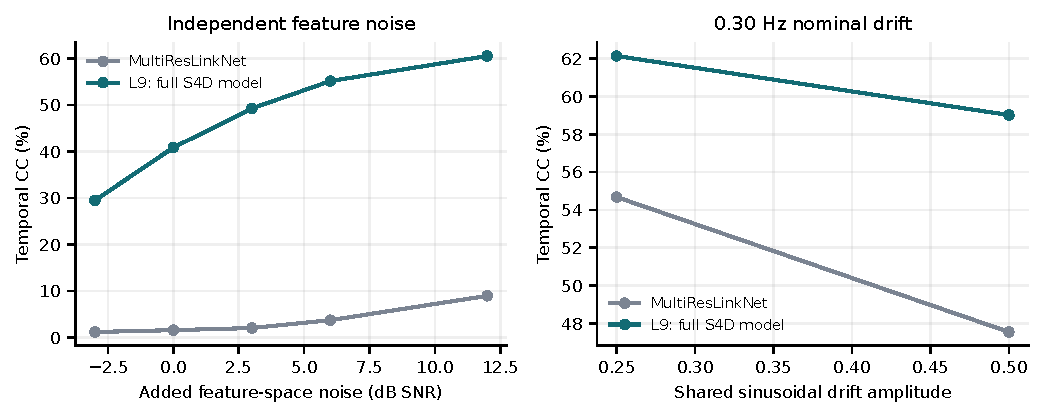
\includegraphics[width=\linewidth]{figures/robustness.pdf}
\caption{Exploratory feature-space stress tests on the first 800 windows of fold 0. Gaussian
noise is independently added to model-input channels after normalisation. The models receive
different noise realisations and different numbers of derived channels. The curves are not
evidence of matched physical sensor-noise robustness across all participants or folds.}
\label{fig:robustness}
\end{figure}

For L9, zeroing the cardiac-band channel reduces temporal correlation to 56.33\%, and
zeroing acceleration reduces it to 58.71\%. Zeroing Q yields 67.27\%, above the clean score.
Such increases can reflect redundancy or input dependence and do not demonstrate that
a channel is harmful when the model is retrained. The phase and displacement channels are
deterministically proportional before normalisation, making redundancy a property of the
representation itself. These results justify a better-controlled robustness study rather
than a physical-noise superiority claim.

\subsection{Compute and training reliability}

Full L9 contains 4,090,620 trainable parameters compared with 9,218,556 for MultiResLinkNet,
a reduction of 55.63\%. No-FiLM and single-task have 4,088,188 and 4,080,698 parameters.
The stored operation counts are 1.245 billion for L9 and 3.478 billion for MultiResLinkNet,
but the coverage caveat prevents interpreting their difference as a verified total-FLOP
reduction. FPN is smaller still, at 2.237 million parameters.

Of the 100 experimental runs, 58 recorded at least one numerical recovery, with 78 events
in total. Twenty runs ended with automatic mixed precision disabled. All 30 LOSO runs
experienced recovery. Completed epoch counts range from 40 to 150, with median 68.5.
These observations show that the recovery mechanism preserved completion, while also
showing that optimisation stability was a material part of the experiment. Process-level
resumption and numerical validity do not establish invariance to precision or recovery
policy.

\section{Discussion}

\subsection{What improves, and what the improvement means}

The main positive result is that the compact S4D family produces competitive reconstruction
under the implemented subject-wise protocol. It improves mean correlation and event agreement
over the MultiResLinkNet rerun with less than half its parameter count. However, the raw
headline difference exaggerates the uniformity of the benefit. MultiResLinkNet's weak fold,
the separation between median and mean participant effects, and the loss of significance
after correction all argue against presenting the average gain as universal improvement.
The comparison with FPN further shows that parameter efficiency is relative to a chosen
baseline rather than an intrinsic property of the new architecture.

The failed reproduction gate is scientifically relevant but not causally diagnostic. It
may reflect the subject split, model details, target transformations, training behaviour
or preprocessing. Establishing which factor is responsible would require controlled reruns
that change one factor at a time. This paper therefore reports the gate as an unresolved
reproduction discrepancy. It does not attribute the gap to errors in the original study.

\subsection{Why more components did not produce a better model}

Both no-FiLM and single-task outperform the full network in mean correlation, and the
single-task contrast survives the specified correction. One plausible explanation is that
noisy auxiliary targets create competing gradients or introduce unreliable conditioning
into the waveform pathway. The detector-derived heatmap is not an independently annotated
target, and its errors can influence both the auxiliary task and the waveform through FiLM.
However, gradient conflict was not directly measured, so this remains a hypothesis rather
than a demonstrated mechanism.

The single-task variant still uses peak-weighted waveform loss. Its advantage therefore
does not show that peak information is unhelpful; it shows that the extra prediction heads
and conditioning pathway did not improve the selected outcome under the present settings.
Similarly, the small lifting ablation effect does not disprove multiresolution learning.
The convolutional branch already represents multiple scales, and the two paths may provide
overlapping information. A carefully tuned lifting-only model could behave differently.

L8 is the best observed correlation variant, but selecting it after inspecting the complete
ladder makes that choice retrospective. Fresh seeds, a fixed model-selection rule and an
independent validation dataset would be needed before advancing it as a confirmed winner.
The appropriate design lesson is to test simpler alternatives explicitly, not to replace
one unconfirmed architectural claim with another.

\subsection{Waveform similarity is insufficient for physiological validity}

The disagreement between correlation rankings and MAE/MSE rankings illustrates the need
to specify the intended use. Correlation rewards agreement in shape after centring and
scaling; amplitude error penalises other departures. Neither directly determines the
accuracy of detected beat intervals. Tilt-up provides a clear example: spectral structure
remains relatively similar while temporal alignment is poor.

The archived RMSSD results are particularly limiting. Even before correcting the time
axis, the errors are far above the project's intended physiological threshold. The
reference-derived RMSSD average is approximately 85 nominal ms, whereas the published
resting table reports 12.95~ms \citep{chowdhury2024}. Different populations of windows,
recording aggregation, detection and artifact rules prevent a direct equivalence. The
125-versus-128-Hz discrepancy alone is only a 2.4\% interval scaling effect and cannot
explain this much larger difference. Filtering out implausible RR intervals before taking
successive differences can also bridge gaps in the interval sequence. A clinical HRV
analysis needs verified event locations and a gap-aware, prespecified artifact policy.

\subsection{The role of an implementation audit}

The sampling-rate finding shows why successful notebook execution is not a sufficient
validation criterion. All required runs and result files can exist while a basic physical
unit is misrepresented. Here, the flaw is independently visible in source logic, raw
sampling metadata and every retained recording length. The correct next step is to fix
the processing contract and recompute the affected outcomes, while keeping the archived
experiment identifiable. Merely changing plot labels or multiplying reported errors would
leave the detector's rate-dependent behaviour unexamined.

The architecture-name audit is similarly consequential. A static S4D kernel cannot be
described as an input-dependent Mamba mechanism, and FFT convolution does not justify a
measured linear-time claim. The code also does not establish complete operation-counter
coverage or warmed-up latency. These distinctions reduce unsupported claims without
discarding the observations that remain valid, especially within-corpus waveform rankings.

\subsection{Limitations and next experiments}

The cohort is small, healthy and acquired with one radar configuration. It does not
support claims about arrhythmia detection, diagnostic morphology, patients in critical
care, other radar hardware or clinical equivalence. Each fold uses one seed, and the
post-hoc bootstrap is conditional on the completed fits. Numerical recoveries and multiple
engine revisions add uncertainty to comparisons. Baseline and experimental training
protocols are not identical, so improvements cannot be attributed solely to architecture.
The condition-held-out protocol permits participant overlap, and the stress test covers
one ordered subset of one fold with unmatched noise realisations.

The highest-priority follow-up is to regenerate or correctly interpret the signal time
base and rerun peak/HRV evaluation with manually checked reference events. A prospective
confirmation should then compare fixed full, no-FiLM and single-task variants using
multiple seeds and stable precision settings. Physical robustness should perturb raw
quadratures with the same realisation for each comparator before recomputing all derived
channels. Fold-complete robustness, an independent dataset, audited computational
profiling and a matched-optimisation baseline would strengthen the eventual submission.

\section{Conclusion}

A completed 180-run campaign provides evidence that compact bidirectional S4D variants can
improve radar-to-ECG reconstruction relative to a strict MultiResLinkNet reimplementation.
The evidence does not validate the full architecture as the best variant: removing FiLM
gives the largest mean correlation, and the single-task model exceeds the full model in
the multiplicity-adjusted participant comparison. Large nominal HRV errors, poor Tilt-up
transfer and a verified time-base discrepancy prevent clinical interpretation of the
archived outputs. The study supports simpler models and more explicit auditing as the
next research direction, with waveform, event and physiological claims evaluated on
their own evidence.

\section*{Data and code availability}

The original data are described by Schellenberger et al.\ \citep{schellenberger2020} and
available through \url{https://doi.org/10.6084/m9.figshare.12186516}. The processed corpus,
run artifacts and evaluation outputs are publicly archived under the Hugging Face account
\texttt{Shanmuk4622}; Appendix~\ref{app:provenance} provides immutable revisions. The
manuscript package contains its analysis code, generated tables, vector figures and a
download manifest for the additional evidence. The repository releases contain the
computational artifacts rather than a clinical certification of their outputs.

\section*{Ethics and consent}

This work reanalyses publicly shared pseudonymised recordings and does not recruit new
participants. The original acquisition study reports approval by the ethics committee of
Friedrich-Alexander-Universit\"at Erlangen-N\"urnberg (No.~85\_15B) and written consent,
including permission to share pseudonymised data \citep{schellenberger2020}. This statement
describes the original study's approval and does not assert a new institutional exemption.

\section*{Funding}\blankfield
\section*{Competing interests}\blankfield
\section*{CRediT authorship contribution statement}\blankfield
\section*{Acknowledgements}\blankfield
\section*{Declaration of generative AI assistance}
Generative AI assisted preparation of the manuscript text and analysis code. The final
author team is responsible for reviewing the manuscript, verifying its claims and
references, and approving the submitted version. Author-specific declarations have been
left blank in this working manuscript.

\FloatBarrier
\bibliographystyle{unsrtnat}
\bibliography{references}

\clearpage
\appendix
\section{Detailed experimental specification}
\label{app:spec}

\begin{longtable}{>{\raggedright\arraybackslash}p{.18\linewidth}>{\raggedright\arraybackslash}p{.72\linewidth}}
\caption{Variant mapping to repository identifiers.}\label{tab:variants}\\
\toprule Identifier & Implemented change\\\midrule\endfirsthead
\toprule Identifier & Implemented change\\\midrule\endhead
L2 & \texttt{L2\_loss\_only}: single displacement input, MultiResLinkNet backbone, composite loss under the experimental training protocol.\\
L3 & \texttt{L3\_c1\_only}: eight inputs, MultiResLinkNet backbone, MSE under the experimental training protocol.\\
L4 & \texttt{L4\_c1\_c5}: eight inputs, MultiResLinkNet backbone, composite loss.\\
L5 & \texttt{L5\_no\_wavelet}: full experimental model without the learned lifting branch and associated fusion.\\
L6 & \texttt{L6\_no\_ssm}: S4D bottleneck replaced by two convolution--normalisation--activation blocks.\\
L7 & \texttt{L7\_singletask}: waveform output only; no peak head, RR head or FiLM; peak-weighted waveform loss remains active.\\
L8 & \texttt{L8\_no\_film}: waveform, peak and RR heads retained; peak-conditioned FiLM removed.\\
L9 & \texttt{L9\_full}: all implemented components.\\
L10 & \texttt{L10\_transformer}: Transformer bottleneck replaces S4D; other full-model components retained.\\\bottomrule
\end{longtable}

The input representation deliberately contains redundancy: displacement is a constant
multiple of unwrapped phase before training-statistic normalisation. The raw quadratures
and amplitude preserve information that the demodulated channel can discard, but their
individual value is not identified by zeroing one channel at inference. A causal feature
assessment would train a fresh model for each retained subset under matched conditions.

For the STFT objective, let $Y_m$ and $\widehat Y_m$ denote magnitude spectra at resolution
$m\in\{64,128,256\}$. The implemented loss is
\begin{equation}
\mathcal L_{\mathrm{STFT}}=\frac13\sum_m\left[
\frac{\|Y_m-\widehat Y_m\|_F}{\|Y_m\|_F+\epsilon}
+\operatorname{mean}\left|\log(Y_m+\epsilon)-\log(\widehat Y_m+\epsilon)\right|
\right].
\end{equation}
Spectral magnitudes are clamped before the logarithm. The peak-weighted term is
\begin{equation}
\mathcal L_{\mathrm{pw}}=
\frac{\sum_n(1+4p_n)|y_n-\hat y_n|}{\sum_n(1+4p_n)+\epsilon}.
\end{equation}
Auxiliary peak logits use focal binary cross-entropy with soft heatmap targets. This is
a surrogate objective for event localisation, not a likelihood derived from independently
adjudicated beat annotations. The RR head uses a softplus output and absolute error in
nominal seconds. Physiology in Table~\ref{tab:clinical} is computed from reconstructed
waveforms, not directly from the auxiliary RR head.

\section{Timing audit and correction boundaries}
\label{app:timing}

The raw inventory records 2,000~Hz for both radar and ECG in all 135 files. Each retained
processed length equals $\lceil N/16\rceil$; none corresponds to exact rational resampling
to 128~Hz. For example, a raw recording with 293,800 samples has 18,363 retained samples,
matching integer decimation by 16. The physical 125-Hz duration is approximately 146.904~s,
while the stored 128-Hz interpretation is approximately 143.461~s.

If event indices were held fixed and no threshold decisions changed, interval quantities
would obey
\begin{equation}
RR_{125}=RR_{128}\frac{128}{125}=1.024\,RR_{128},
\qquad HR_{125}=HR_{128}\frac{125}{128}.
\end{equation}
The same interval factor would apply to RMSSD computed from an unchanged retained-interval
sequence. This implies a 2.4\% increase in intervals and a 2.34375\% decrease in HR relative
to the archived values. It does not justify a corrected physiological result, because
rerunning the detector at 125~Hz changes its digital filter, smoothing, refractory period
and acceptance thresholds. The interval-filtering rule can also retain a different set
of intervals.

At the current detector settings, nominal 100-ms matching spans 12.8 samples, equivalent
to 102.4 physical milliseconds. The nominal 5--25-Hz filter acts on approximately
4.883--24.414 physical Hz. The 1,024-sample window is 8.192~s and the training hop is
4.096~s. These differences are small compared with the observed RMSSD errors but are
systematic and must be resolved in any physically calibrated evaluation.

An exact 128-Hz rebuild would use an appropriate rational resampler with ratio $8/125$
from the 2,000-Hz source. Alternatively, retaining the existing 125-Hz stream would require
updating all dependent sampling assumptions and defining the changed window duration.
Either choice needs a new, explicit processed-data revision. This manuscript does not
report unperformed rebuilding or reevaluation as completed work.

\section{Aggregation, uncertainty and reporting safeguards}

The three principal aggregation rules answer different questions. The headline waveform
table averages windows within fold and then averages five folds equally. Participant-paired
statistics average all held-out windows within each participant. The physiological table
first averages recordings within participant, then gives all participants equal weight.
Consequently, a participant with more recordings or a longer recording can influence one
table differently from another. The difference between the full-model RMSSD errors of
200.83 in the original fold-summary ablation table and 201.42 in the participant-level
table is an aggregation difference, not evidence that one run was overwritten.

The saved peak-count columns in the notebook-level table are sums of participant-level
recording averages. They are not integer pooled TP/FP/FN totals. We therefore do not
present those columns as micro-averaged event counts. The reported F1 is macro-averaged
from the stated units of analysis and is not recomputed from those averaged counts.

For the added bootstrap, the unit resampled is the paired participant difference. In each
replicate, 30 differences are sampled with replacement and their arithmetic mean is
computed. The 2.5th and 97.5th percentiles give the reported interval. The analysis is
conditional on these trained models: it does not refit the networks, propagate
preprocessing uncertainty or compensate for selecting L8 after reviewing the ladder.

The signed-rank family is exactly the one retained in the archived NB05 output. Its nine
uncorrected probabilities and adjusted values were reproduced to numerical tolerance
$10^{-12}$. This verifies faithful calculation from the archive; it does not turn a
retrospective benchmark into a prospective trial or remove dependence from overlapping
training sets. The results should therefore be read as evidence about this campaign.

The operation counter records 1.245 billion operations for full L9, 1.240 for no-FiLM,
1.225 for single-task, 1.301 for the Transformer variant and 3.478 for MultiResLinkNet.
Until FFT and complex-kernel operation coverage is audited, these values are lower-level
profiling observations. First-call latency records range from tens to more than a thousand
milliseconds across variants and do not provide a trustworthy deployment benchmark.

\section{Provenance and reproducibility package}
\label{app:provenance}

The public namespace is \texttt{Shanmuk4622}. The evidence freeze uses the following revisions:
\begin{description}[style=nextline]
\item[Evaluation: \texttt{cardiomamba-results-v2}]
\path{bb25560143d1044dc8671ef487160cc0049f7282}
\item[Experimental models: \texttt{cardiomamba-net-v2}]
\path{dd5764c51031f5d9415ecddbe64ff10ab0d02348}
\item[Baselines: \texttt{cardiomamba-baselines-v2}]
\path{84bf3e7992a33aecacfb30ab860872c620ca7699}
\item[Processed dataset: \texttt{cr-rvs-radar-ecg-processed-v2}]
\path{be14c2a90442d38235c5095d7d4eac07dfa9adcd}
\item[Raw inventory: \texttt{cr-rvs-radar-ecg-inventory-v2}]
\path{ef9d72a2dbe5e185644be0c8cd44bb13ab2f3727}
\end{description}

The first three are model-type Hugging Face repositories and the latter two are dataset-type
repositories. The final evaluation status is \texttt{inputs-complete-gate-failed}: all expected
inputs were present, while the baseline reproduction requirement failed. It is not a
statement that the experiment was scientifically validated.

The local snapshot preserves 612 downloaded artifacts, including all canonical run
summaries, configurations and environment records, the final tables and figures, processed
indexes and five primary full-model checkpoints. The manuscript-specific evidence adds 99
files, with URLs and SHA-256 hashes in a separate download manifest. Every primary model
has 6,278 per-window results, covering the same 30 participants.

Hashes for the archived experimental model, data, loss, metrics and baseline-model modules
match the values recorded in all 45 primary experimental run configurations. The latest
archived experimental engine matches only one of these 45 configurations, demonstrating
engine-version turnover during the campaign. All 20 primary baseline configurations match
their archived baseline engine. Exact replay therefore requires resolving the engine
revision recorded by each run, rather than assuming that the repository's latest engine
is the one that trained every checkpoint.

The package includes \texttt{main.tex}, a checked BibTeX database, generated table rows,
vector figures, conditional-bootstrap results, the 134-recording time-base audit and the
analysis script that regenerates these assets from the frozen evidence. Scientific
results are sourced from archived outputs; editorial prose and figure layouts were
prepared specifically for this manuscript.

\clearpage
\section{Matched waveform examples}
\label{app:qualitative}

Figure~\ref{fig:qualitative} uses the saved fold-0 prediction sample. The training worker
retains up to 200 equally spaced indices from its test-window sequence. We rank those
saved windows by full-model temporal correlation and select the windows at the integer
rank positions nearest below the 25th, 50th and 75th percentiles. This deterministic rule
samples a range of outcomes rather than choosing a visually favourable reconstruction.
It remains a selection based on one model's scores, not a random sample of the full corpus.

For every displayed row, the reference arrays and participant identifiers match exactly
across MultiResLinkNet, full L9 and no-FiLM after conversion to the common target scale.
The source index, participant and computed correlation for every panel are retained in
the manuscript's generated evidence. The time axis uses the audited physical rate of
125~Hz, while the underlying saved predictions are unchanged. These panels illustrate
the differences between models on individual traces; they do not add statistical tests.

\begin{figure}[htbp]\centering
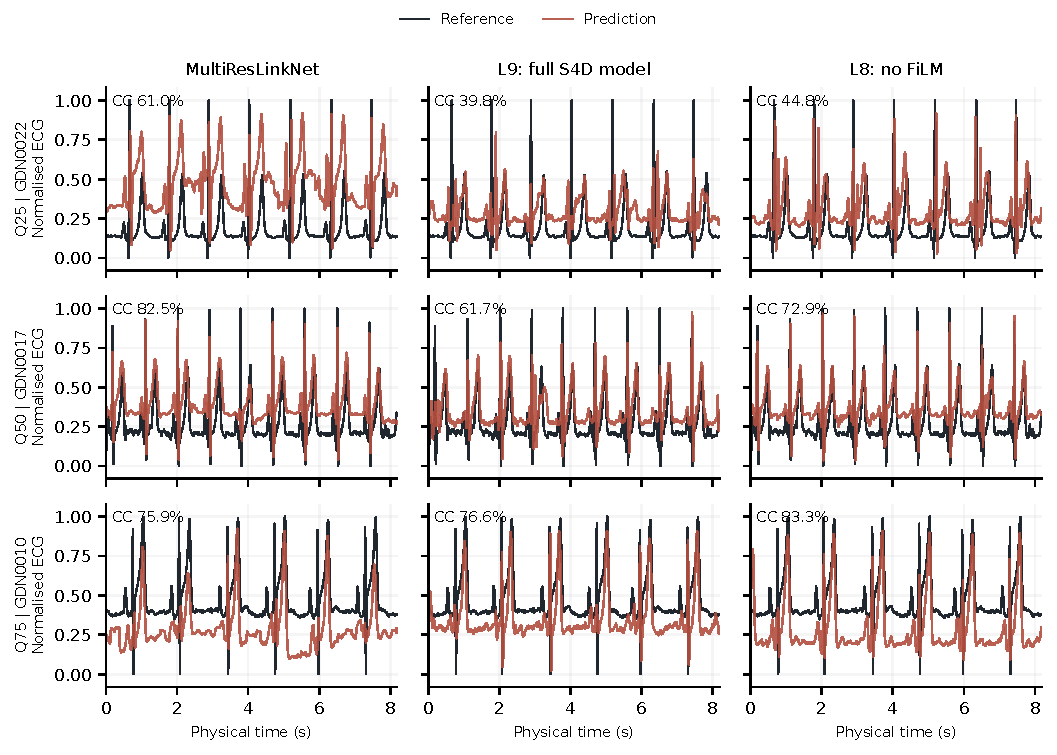
\includegraphics[width=\linewidth]{figures/qualitative.pdf}
\caption{Matched fold-0 waveform examples. Rows correspond to approximately the 25th, 50th
and 75th percentiles of full-model correlation within the saved sample. Columns show
MultiResLinkNet, full L9 and no-FiLM. Black is the reference and red is the reconstruction.
The vertical scale is the shared normalised $[0,1]$ target convention; horizontal axes
show physical time at 125~Hz. The displayed CC values are recomputed directly from the
saved arrays.}
\label{fig:qualitative}
\end{figure}

\end{document}
